\documentclass{beamer}\usepackage{graphicx, color}
%% maxwidth is the original width if it is less than linewidth
%% otherwise use linewidth (to make sure the graphics do not exceed the margin)
\makeatletter
\def\maxwidth{ %
  \ifdim\Gin@nat@width>\linewidth
    \linewidth
  \else
    \Gin@nat@width
  \fi
}
\makeatother

\IfFileExists{upquote.sty}{\usepackage{upquote}}{}
\definecolor{fgcolor}{rgb}{0.2, 0.2, 0.2}
\newcommand{\hlnumber}[1]{\textcolor[rgb]{0,0,0}{#1}}%
\newcommand{\hlfunctioncall}[1]{\textcolor[rgb]{0.501960784313725,0,0.329411764705882}{\textbf{#1}}}%
\newcommand{\hlstring}[1]{\textcolor[rgb]{0.6,0.6,1}{#1}}%
\newcommand{\hlkeyword}[1]{\textcolor[rgb]{0,0,0}{\textbf{#1}}}%
\newcommand{\hlargument}[1]{\textcolor[rgb]{0.690196078431373,0.250980392156863,0.0196078431372549}{#1}}%
\newcommand{\hlcomment}[1]{\textcolor[rgb]{0.180392156862745,0.6,0.341176470588235}{#1}}%
\newcommand{\hlroxygencomment}[1]{\textcolor[rgb]{0.43921568627451,0.47843137254902,0.701960784313725}{#1}}%
\newcommand{\hlformalargs}[1]{\textcolor[rgb]{0.690196078431373,0.250980392156863,0.0196078431372549}{#1}}%
\newcommand{\hleqformalargs}[1]{\textcolor[rgb]{0.690196078431373,0.250980392156863,0.0196078431372549}{#1}}%
\newcommand{\hlassignement}[1]{\textcolor[rgb]{0,0,0}{\textbf{#1}}}%
\newcommand{\hlpackage}[1]{\textcolor[rgb]{0.588235294117647,0.709803921568627,0.145098039215686}{#1}}%
\newcommand{\hlslot}[1]{\textit{#1}}%
\newcommand{\hlsymbol}[1]{\textcolor[rgb]{0,0,0}{#1}}%
\newcommand{\hlprompt}[1]{\textcolor[rgb]{0.2,0.2,0.2}{#1}}%

\usepackage{framed}
\makeatletter
\newenvironment{kframe}{%
 \def\at@end@of@kframe{}%
 \ifinner\ifhmode%
  \def\at@end@of@kframe{\end{minipage}}%
  \begin{minipage}{\columnwidth}%
 \fi\fi%
 \def\FrameCommand##1{\hskip\@totalleftmargin \hskip-\fboxsep
 \colorbox{shadecolor}{##1}\hskip-\fboxsep
     % There is no \\@totalrightmargin, so:
     \hskip-\linewidth \hskip-\@totalleftmargin \hskip\columnwidth}%
 \MakeFramed {\advance\hsize-\width
   \@totalleftmargin\z@ \linewidth\hsize
   \@setminipage}}%
 {\par\unskip\endMakeFramed%
 \at@end@of@kframe}
\makeatother

\definecolor{shadecolor}{rgb}{.97, .97, .97}
\definecolor{messagecolor}{rgb}{0, 0, 0}
\definecolor{warningcolor}{rgb}{1, 0, 1}
\definecolor{errorcolor}{rgb}{1, 0, 0}
\newenvironment{knitrout}{}{} % an empty environment to be redefined in TeX

\usepackage{alltt}
\usetheme{Stats}
\setbeamercovered{transparent}
\usepackage{color}
\usepackage{hyperref}
  \hypersetup{
  	colorlinks=true
		linkcolor=black
		}
\usepackage{url}
\usepackage{graphics}
\usepackage{tikz}
\usepackage{booktabs}





%%%%%%%%%%%%%%%%%%%%%%%%%%%%%%%% Title Slide %%%%%%%%%%%%%%%%%%%%%%%%%%
\title[]{Intro to Social Science Data Analysis \\[1cm] Lecture 4: Replication! }
\author[]{
    \href{mailto:gandrud@yonsei.ac.kr}{Christopher Gandrud}
}
\date{\today}


\begin{document}

\frame{\titlepage}

\section[Outline]{}
\frame{\tableofcontents}

\section{Recap}
\frame{
	\frametitle{Recap}
  {\LARGE{Last class we discussed:}}
  \begin{itemize}
    \item populations \& samples,
    \item random samples \& convenience samples,
    \item response, explanatory, and control variables,
    \item importing data into R,
    \item merging data sets.
  \end{itemize}
}

\frame{
  \frametitle{Review Quiz (1)}
  Imagine you have a data set in a \texttt{.csv} file on your desktop. \\[0.5cm]
  Describe the steps you would take to import the data set into R.
}

\frame{
  \frametitle{Review Quiz (2)}
  \begin{enumerate}
    \item What is the difference between a population and a sample?
    \item What do you need to be honest about when using convenience samples?
  \end{enumerate}
}

\begin{frame}[fragile]
  \frametitle{Review Quiz (3)}
  Comment the code:
  
\begin{knitrout}
\definecolor{shadecolor}{rgb}{0.969, 0.969, 0.969}\color{fgcolor}\begin{kframe}
\begin{alltt}
\hlcomment{#}
\hlfunctioncall{library}(reshape) 

\hlcomment{#}
Data <- \hlfunctioncall{rename}(Data, \hlfunctioncall{c}(country_name = \hlstring{"Country"}))

\hlcomment{#}
Data$Country[Data$Country 
             == \hlstring{"Dem. Rep. Congo"}] <- \hlstring{"DRC"}
\end{alltt}
\end{kframe}
\end{knitrout}


\end{frame}

\frame{
  Now we know how to get data into R in a format we can use for statistical analysis. \\[0.5cm]
  Before we start analysing the data, it is important to learn another computational research skill \ldots
}

\frame{
  \begin{center}
    {\LARGE{Reproducible Research}}
  \end{center}
}

%%%%%%%%%%%%% What is reproducible research?
\section{What is reproducible research?}
\frame{
  \frametitle{What is replicable research?}
  {\LARGE{Replicable Research}} \\[0.5cm]
  Research is replicable if {\emph{there is sufficient information for independent researchers to make the same findings using the same procedures}} (King 1995, 444).
}

\frame{
  {\LARGE{For example,}}
  A team of scientists clone a sheep. \\[0.5cm]
  The team documents the prodedures they use to clone the sheep and make these procedures available on their website. \\[0.5cm]
  Another team of scientists is able to use the information on the website to clone another sheep.
}

\frame{
  \frametitle{What is reproducible research?}
  {\LARGE{Reproducible Research}} \\[0.5cm]
  Reproducible reasearch is when {\emph{the data and code used to make a finding are available and they are sufficient for an independent researcher to make the same findings (see Peng 2011).}} \\[0.5cm]
}

\frame{
  \frametitle{Why reproducible, not replicable?}
  Sometimes with observational data it may require too many resources to gather a new set of data or, especially in the case of cross-country data it may not be possible to gather other data. \\[0.5cm]
  So, reproducibility can be a {\bf{second-best}} if replicability is difficult.
}

\frame{
  \frametitle{What is research?}
  A book, an article, or a research paper is {\bf{not research}}. \\[0.5cm]
  It is an {\bf{advertisment}} for the research. \\[0.5cm]
  The research is ``the {\bf{full software environment, code, and data}} that produced the results" (Buckheit and Donoho, 1995; Donoho, 2010, 385)
}

\frame{
  \frametitle{Doing reproducible computational research.}
  \begin{center}
    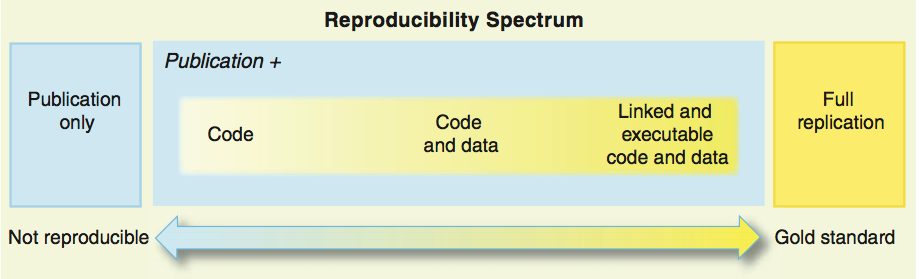
\includegraphics[scale = 0.35]{RepSpectrum.png} \\[0.75cm]
    {\small{Peng (2011, 1226)}}
  \end{center}
}


%%%%%%%%%%%%% Why do reproducible research?
\section{Why do reproducible research?}
\frame{
  \begin{center}
    {\LARGE{Why do reproducible research?}}
  \end{center}
}

\frame{
  \begin{center}
    {\LARGE{In this class I require you to.}}
  \end{center}
}

\frame{
  \begin{center}
    {\LARGE{Reproducible research is a key part of science.}}
  \end{center}
}

\frame{
  \frametitle{Reproducible research \& science}
  Braude (1979, 2) has even called replication the ``demarcation between science and non-science."
}

\frame{
  \frametitle{What is science?}
  {\LARGE{Science}} \\[0.5cm]
  The ``systematic enterprise of gathering knowledge about the universe and organizing and condensing that knowledge into {\bf{testable}} laws and theories`` \\[0.5cm]
  {\small{(see APA \url{http://www.aps.org/policy/statements/99_6.cfm})}}
}

\frame{
  \frametitle{Replication \& Science}
  Scientists need to ``{\bf{expose}} their ideas and results to independent testing and replication by others. \\[0.25cm]
  This requires the {\bf{open exchange of data, procedures and materials}}."\\[0.5cm]
  {\small{(Emphasis added, see APA \url{http://www.aps.org/policy/statements/99_6.cfm})}}
}

\frame{
  \frametitle{Avoiding effort duplication}
  Making your data and procedures available also helps avoid {\bf{effort dublication}}. 
    \begin{itemize}
      \item Others don't have to gather the same data or figure out the same analysis that you have already done.
    \end{itemize} \\[0.5cm]
  This helps build {\bf{cumulative scientific knowledge}}.
}

\frame{
  \begin{center}
    {\LARGE{Reproducible research is good for you.}}
  \end{center}
}

\frame{
  As you will see, making your research reproducible requires an extra {\bf{upfront}} investment. \\[0.5cm]
  Beyond the benefits for science, why should you make your research more reproducible?  
}

\frame{
  \frametitle{Why reproducible research benefits you.}
  {\LARGE{Reproducible research benefits for you:}}
  \begin{itemize}
    \item Better work habits.
    \item Better teamwork.
    \item Making changes is easier.
    \item Higher research impact.
  \end{itemize}
}

\begin{frame}[fragile]
  We have {\emph{already started}} doing reproducible research. 
  \begin{itemize}
  \item<1-> You have already been making your code human readable with comments after the \texttt{\#}.
  \item<2-> You have been compiling notebooks of your code and output.
  \end{itemize}
\end{frame}

\frame{
  So far we have mostly focused on the source code. \\[0.5cm]
  Today we will learn how to {\bf{weave}} the source code and presentation documents together.
}

\frame{
  First, we will learn the basics of the {\bf{Markdown}} markup language. \\[0.5cm]
  Second, we will learn how to use the {\emph{knitr}} package to weave our {\emph{source code}} and {\emph{Markdown presentation documents}}.
}

\frame{
  \frametitle{Doing reproducible computational research.}
  To be ``really reproducible" we need a way to {\bf{{\emph{link}} the data, code, and presentation}} documents. \\[1cm]
  The {\emph{knitr}} package for R is this link. \\[0.5cm]
  \begin{itemize}
    R Source Code $\Longleftrightarrow$ knitr package $\Longleftrightarrow$ Markdown  
  \end{itemize}
}

%%%%%%%%%%%%% Doing Reproducible Research: Markup languages 
\section{Doing reproducible research: markup languages}
\frame{
  \begin{center}
    {\LARGE{The Markdown Markup Language.}}
  \end{center}
}

\frame{
  \frametitle{What is a markup language?}
  {\LARGE{Markup Language}} \\[0.5cm]
  Instructions for how to format a presentation document. \\[0.5cm]
  You are probably familiar with the HTML markup language used to create websites.
}

\frame{
  \frametitle{HTML is a Pain!}
  \begin{center}
    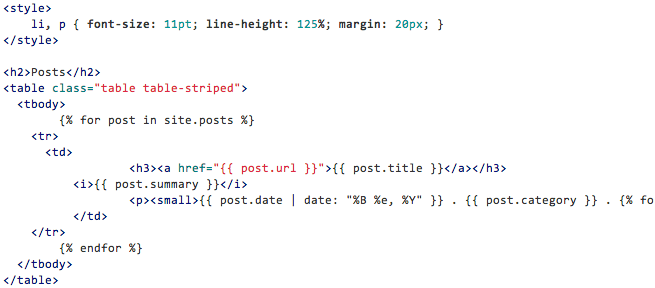
\includegraphics[scale = 0.5]{htmlExample.png}
  \end{center}
}

\frame{
  \frametitle{What is the Markdown markup language?}
  {\LARGE{Markdown}} \\[0.5cm]
  The Markdown markup language {\emph{simplifies}} the process of creating HTML markup files. \\[0.5cm]
  Markdown files have the file extension: \texttt{.md} or \texttt{.markdown}.
}

\frame{
  \frametitle{Markdown \textrightarrow\: HTML}
  \begin{center}
    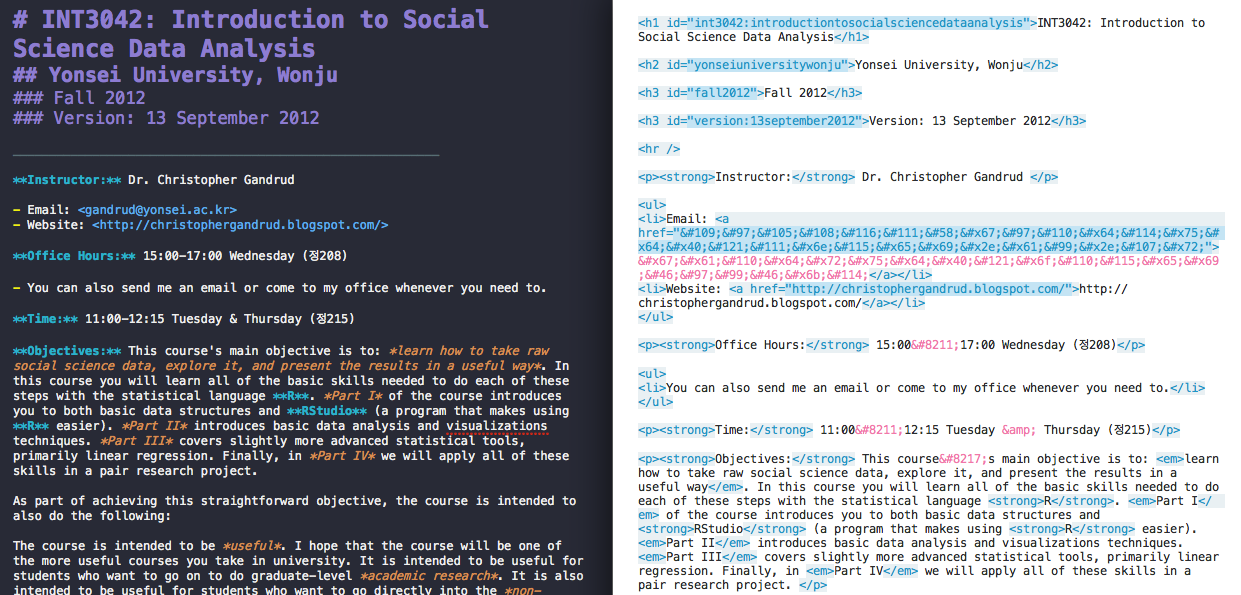
\includegraphics[scale = 0.3]{markdownTohtml.png}
  \end{center}  
}

\frame{
  \frametitle{Final}
  \begin{center}
    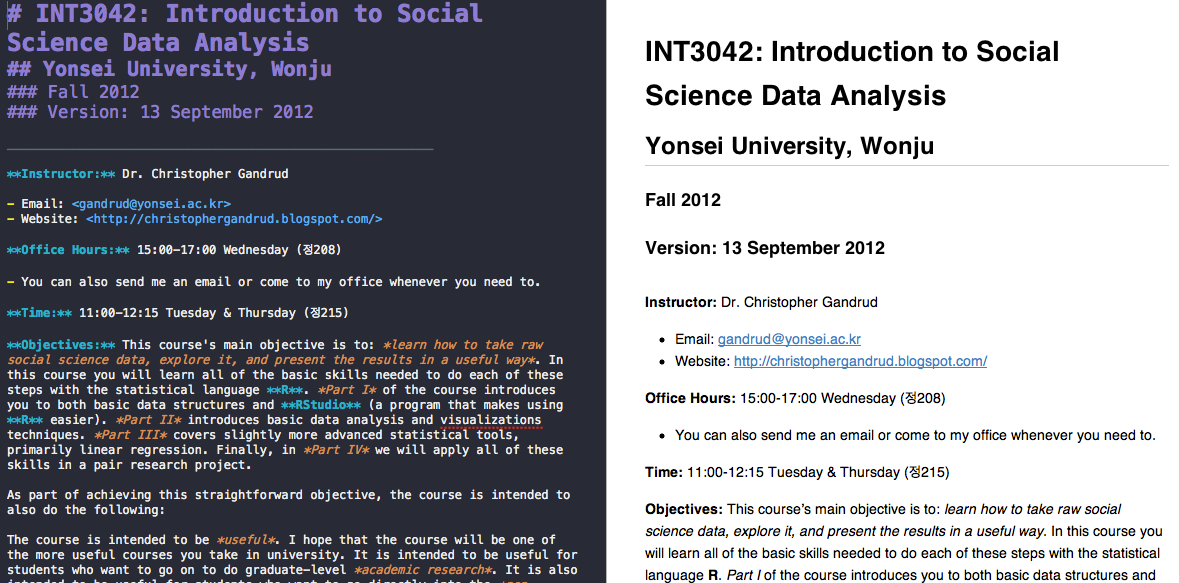
\includegraphics[scale = 0.3]{SyllabusSnap.png}
  \end{center}  
}

\frame{
  \frametitle{Basic Markdown Syntax}
  You can find a guide to basic Markdown Syntax at:
    \begin{itemize}
      \item {\small{\url{http://daringfireball.net/projects/markdown/basics}}}      
    \end{itemize} \\[0.5cm]
    Also, {\bf{anything}} you can do in HTML you can do in Markdown.
}

\frame{
  \frametitle{Programs for editing markdown documents}
  {\LARGE{Free programs for editing markdown documents}} \\[0.5cm]
  \begin{itemize}
    \item {\bf{Mac:}} Mou (\url{http://mouapp.com/}).
    \item {\bf{Windows:}} MarkdownPad (\url{http://markdownpad.com/}).
  \end{itemize} \\[0.5cm]
  These programs allow you to create webpages \& PDFs. \\[0.5cm]
  You can host HTML pages from your Dropbox Public Folder
}

\frame{
  \frametitle{R Markdown}
  If we want to combine R code and Markdown we can use RStudio. \\[0.5cm]
  To create a new R Markdown document: \\[0.5cm]
  \begin{center}
    \texttt{File} \textrightarrow\: \texttt{New}\textrightarrow\: \texttt{R Markdown}
  \end{center} \\[0.5cm]
  R Markdown documents have the file extension \texttt{.Rmd}. 
}

\frame{
  \frametitle{The RStudio Markdown Top Bar, Left Side}
  {\LARGE{Open a new R Markdown document \& play with these buttons in RStudio.}} \\[1cm]
  \begin{center}
    
\includegraphics[scale = 0.5]{MarkdownTopBarLeft.png}
  \end{center} \\[1cm]
  {\large{What do they do?}}
}

%%%%%%%%%%%%% Doing Reproducible Research: knitr 
\section{Doing reproducible research: knitr}
\frame{
  Now that we understand the basics of the Markdown markup language, lets start ``{\bf{knitting}}" R code into our presentation documents.
}

\frame{
  \frametitle{The ``Knit HTML" Button}
  CLicking on the ``Knit HTML" button (\raisebox{-2mm}{
\includegraphics[scale=0.75]{KnitHTMLButton.png}}):
  \begin{itemize}
    \item Runs the R {\bf{code chunks}},
    \item Puts the output into a new plain Markdown file (\texttt{.md}),
    \item Converts the Markdown file to HTML.
  \end{itemize}
}

\frame{
  \frametitle{What is a code chunk?}
  {\LARGE{Code Chunks}} \\[0.5cm]
  We place R code inside of code chunks, this seperates them from the markup and text. \\[0.5cm]
  Knitr looks for code chunks and runs the code in them. 
}

\begin{frame}[fragile]
  \frametitle{Code Chunk Syntax}
  {\LARGE{Knitr/Markdown Code Chunk Syntax}}
\begin{knitrout}
\definecolor{shadecolor}{rgb}{0.969, 0.969, 0.969}\color{fgcolor}\begin{kframe}
\begin{alltt}
\hlcomment{# A Knitr/Markdown code chunk starts like this}
```\{r\}
\end{alltt}
\end{kframe}
\end{knitrout}


\begin{knitrout}
\definecolor{shadecolor}{rgb}{0.969, 0.969, 0.969}\color{fgcolor}\begin{kframe}
\begin{alltt}
\hlcomment{# A Knitr/Markdown code chunk ends like this}
```
\end{alltt}
\end{kframe}
\end{knitrout}

\end{frame}

\frame{
  \frametitle{Chunk Options}
  {\LARGE{Chunk Options}} \\[0.5cm]
  You can add options to your chunks to change how they behave.
}

\frame{
  \frametitle{Chunk Options}
  \begin{center}
    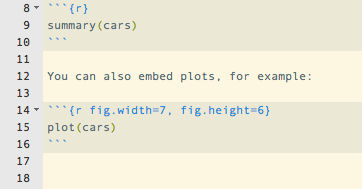
\includegraphics[scale = 0.65]{ChunkRStudioExamples.png}
  \end{center}
}

\begin{frame}[fragile]
  \frametitle{Chunk Options}
  The options:
\begin{knitrout}
\definecolor{shadecolor}{rgb}{0.969, 0.969, 0.969}\color{fgcolor}\begin{kframe}
\begin{alltt}
```\{r fig.width=7, fig.height=6\}
\end{alltt}
\end{kframe}
\end{knitrout}

  Set how wide and tall the output figure is. 
\end{frame}

\frame{
  \frametitle{R Markdown Final}
  \begin{center}
    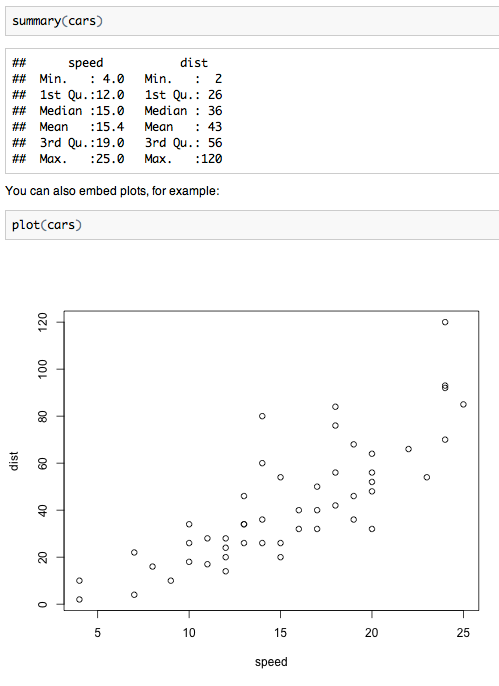
\includegraphics[scale = 0.3]{CarsMarkdown.png}
  \end{center}
}

\frame{
  \frametitle{Useful Chunk Options}
  \begin{table}
  \begin{tabular}{l p{5cm}}
    \hline  
    Chunk Option & Description \\ \hline\hline
    \texttt{eval=FALSE} & Does not run the code \\
    \texttt{echo=FALSE} & Does not include the code \\
    \texttt{error=FALSE} & Does not include error messages \\
    \texttt{warning=FALSE} & Does not include warning messages \\
    \texttt{message=FALSE} & Does not include message messages \\
    \texttt{fig.align='center'} & Centers a figure \\
    \hline
  \end{tabular}
  \end{table}
}

\frame{
  \frametitle{More Chunk Options}
  All chunk options can be found at: \\[0.5cm]
  \begin{itemize}
    \url{http://yihui.name/knitr/options}.
  \end{itemize}
}

\frame{
  If you want well formatted PDF files and slide shows (like this one), especially if you plan to go to graduate school. \\[0.5cm]
  You can learn how to use knitr and \LaTeX. \\[0.5cm]
  See me for more details. \\[0.5cm]
  {\bf{Note:}} \LaTeX markup syntax is more complicated than Markdown. \\ 
  You also do not need to know \LaTeX for this course.
}


\begin{frame}[allowframebreaks]
  \frametitle{References}
  Braude, S.E. ESP and Psychokinesis. A philosophical examination. Temple University Press, Philadelphia, PA, 1979. \\[0.25cm]
  Buckheit, J. B. and Donoho, D. L. (1995). Wavelab and Reproducible Research, pages 55–81. Springer, New York. \\[0.25cm]
  Donoho, D. L. (2010). An Invitation to Reproducible Computational Research. Biostatistics, 11(3):385–388. \\[0.25cm]
  King, Gary. 1995. “Replication, Replication.” PS: Political Science and Politics 28(3): 444–452. \\[0.25cm] 
  Peng, Roger D. 2011. “Reproducible Research in Computational Science.” Science 334:1226-1227.
\end{frame}


\end{document}
